% =============================================================================
\section{PX4 y el x500}
% =============================================================================

\begin{frame}{Idea central}
  \begin{columns}[c]
    \column{0.52\textwidth}
    \begin{idea}
      \textbf{PX4} es el piloto automático: el programa que corre en la controladora de vuelo y
      mantiene al dron en el aire. \textbf{ROS 2} es donde escribimos \emph{la misión}: qué hacer,
      a dónde ir, cuándo aterrizar.
    \end{idea}
    \vspace{0.4em}\small
    Nosotros \textbf{no controlamos los motores}: le pedimos cosas a PX4 (``ve a este punto'',
    ``aterriza'') y leemos lo que nos cuenta (posición, batería, modo).
    \column{0.45\textwidth}\centering
    \begin{tikzpicture}[node distance=0.5cm,every node/.style={font=\scriptsize},
        bx/.style={draw=azul,fill=azulclaro,rounded corners,minimum width=3.2cm,minimum height=0.7cm,align=center}]
      \node[bx,fill=yellow!20] (ros) {Tu nodo de ROS 2\\(la misión)};
      \node[bx,below=0.9cm of ros] (px4) {PX4\\(el piloto)};
      \node[bx,below=0.9cm of px4,fill=gray!15,draw=gray] (mot) {Motores y sensores};
      \draw[-{Stealth},thick] ([xshift=-0.6cm]ros.south) -- node[left]{pide} ([xshift=-0.6cm]px4.north);
      \draw[-{Stealth},thick] ([xshift=0.6cm]px4.north) -- node[right]{cuenta} ([xshift=0.6cm]ros.south);
      \draw[{Stealth}-{Stealth},thick] (px4) -- node[right]{400 Hz} (mot);
    \end{tikzpicture}
  \end{columns}
\end{frame}

\begin{frame}{¿Qué es PX4?}
  \begin{columns}[c]
  \column{0.68\textwidth}
  \begin{itemize}
    \item Un \textbf{autopiloto de código abierto} (BSD) para drones, aviones, VTOL, rovers y más.
    \item Corre en una \textbf{controladora de vuelo} (Pixhawk 6C, 6X, Cube\ldots) con un sistema
      operativo de tiempo real (NuttX).
    \item Por dentro son \textbf{módulos} independientes: sensores, estimador, controladores,
      \cmd{commander} (modos y armado), \cmd{navigator} (misiones), registro\ldots
    \item La misma base de código corre en \textbf{simulación} (SITL) en tu computadora.
    \item Usamos \textbf{PX4 v1.17.0} (fijado en \cmd{vespo.toml}); \cmd{px4\_msgs} tiene que coincidir.
  \end{itemize}
  \column{0.3\textwidth}\centering
  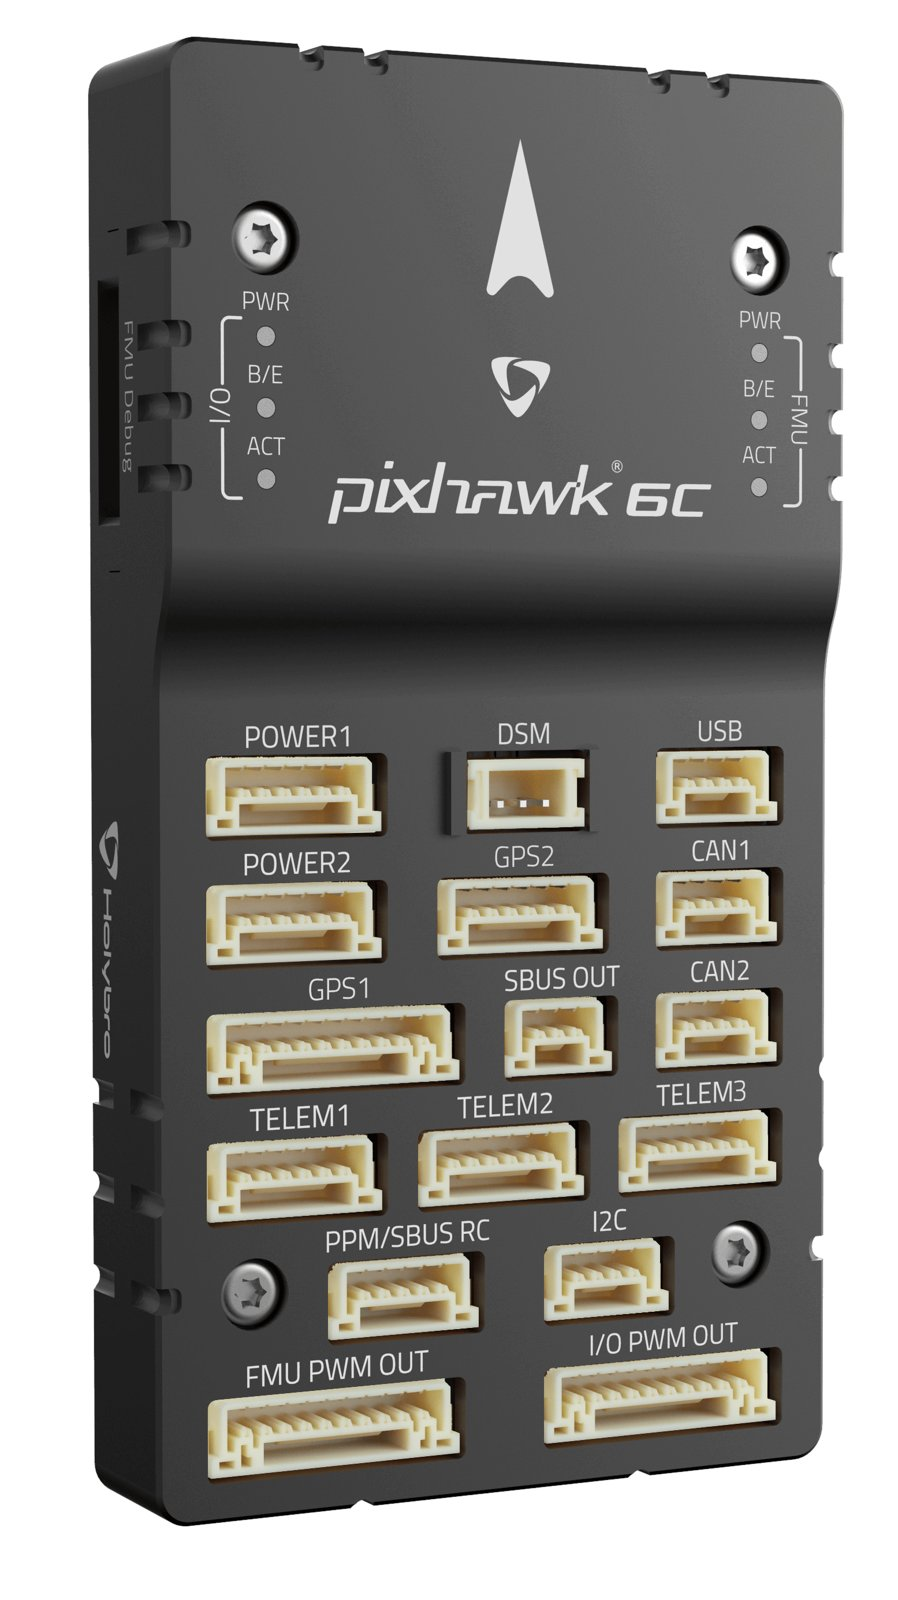
\includegraphics[height=0.55\textheight]{pixhawk6c}\\
  \credito{Pixhawk 6C. Docs de PX4 (CC BY 4.0)}
  \end{columns}
\end{frame}

\begin{frame}{Real contra simulación}
  \begin{columns}[t]
    \column{0.48\textwidth}\centering
    \textbf{En el dron}\\[0.4em]
    \begin{tikzpicture}[node distance=0.35cm,every node/.style={font=\tiny},
        bx/.style={draw=azul,fill=azulclaro,rounded corners,minimum width=2.6cm,align=center}]
      \node[bx] (c) {Computadora a bordo\\(Jetson / Raspberry Pi)\\ROS 2 + agente};
      \node[bx,below=of c] (p) {Pixhawk\\PX4};
      \node[bx,below=of p,fill=gray!15,draw=gray] (m) {ESC + motores, IMU, GPS};
      \draw[{Stealth}-{Stealth}] (c) -- node[right]{serial / USB} (p);
      \draw[{Stealth}-{Stealth}] (p) -- (m);
    \end{tikzpicture}
    \column{0.48\textwidth}\centering
    \textbf{En tu laptop (SITL)}\\[0.4em]
    \begin{tikzpicture}[node distance=0.35cm,every node/.style={font=\tiny},
        bx/.style={draw=azul,fill=azulclaro,rounded corners,minimum width=2.6cm,align=center}]
      \node[bx] (c) {ROS 2 + agente};
      \node[bx,below=of c] (p) {PX4 SITL\\(un proceso: bin/px4)};
      \node[bx,below=of p,fill=gray!15,draw=gray] (m) {Gazebo: física, motores\\y sensores simulados};
      \draw[{Stealth}-{Stealth}] (c) -- node[right]{UDP 8888} (p);
      \draw[{Stealth}-{Stealth}] (p) -- node[right]{gz\_bridge} (m);
    \end{tikzpicture}
  \end{columns}
  \vspace{0.4em}
  \begin{idea}
    \small Tu nodo \textbf{no sabe} si habla con un dron real o con la simulación: los topics son los mismos.
    Por eso todo se prueba primero en SITL.
  \end{idea}
\end{frame}

\begin{frame}{Por dentro: módulos que se hablan por uORB}
  \centering
  \begin{tikzpicture}[node distance=0.4cm,every node/.style={font=\tiny},
      md/.style={draw=azul,fill=azulclaro,rounded corners,minimum width=1.9cm,minimum height=0.55cm,align=center}]
    \node[md] (s) {sensores};
    \node[md,right=of s] (e) {EKF2\\(estimador)};
    \node[md,right=of e] (pc) {control de\\posición};
    \node[md,right=of pc] (ac) {control de\\actitud y rate};
    \node[md,right=of ac] (ca) {control\\allocation};
    \node[md,below=0.8cm of e] (cm) {commander\\(armado, modos)};
    \node[md,below=0.8cm of pc] (nv) {navigator\\(Takeoff, RTL\ldots)};
    \node[md,below=0.8cm of ac,fill=yellow!20] (dds) {uxrce\_dds\_client\\(puente a ROS 2)};
    \draw[-{Stealth}] (s) -- (e); \draw[-{Stealth}] (e) -- (pc); \draw[-{Stealth}] (pc) -- (ac); \draw[-{Stealth}] (ac) -- (ca);
    \draw[-{Stealth},dashed] (nv) -- (pc); \draw[-{Stealth},dashed] (cm) -- (nv);
    \draw[{Stealth}-{Stealth},dashed,naranja] (dds) -- (ac);
  \end{tikzpicture}
  \vspace{0.6em}
  \begin{itemize}\small
    \item \textbf{uORB}: el ``ROS interno'' de PX4. Cada módulo publica y se suscribe a \emph{topics} uORB
      (\cmd{vehicle\_local\_position}, \cmd{battery\_status}\ldots).
    \item El módulo \cmd{uxrce\_dds\_client} copia algunos de esos topics a ROS 2 y trae otros de vuelta.
  \end{itemize}
\end{frame}

\begin{frame}{El x500}
  \begin{columns}[c]
    \column{0.5\textwidth}\small
    \begin{itemize}
      \item Cuadricóptero de Holybro, marco en \textbf{X}, \textasciitilde500 mm de motor a motor en diagonal.
      \item Es el modelo por defecto de PX4 en Gazebo (\cmd{gz\_x500}, airframe \cmd{4001}).
      \item Variantes de PX4 con sensores: \cmd{x500\_lidar\_2d}, \cmd{x500\_mono\_cam\_down},
        \cmd{x500\_depth}\ldots
      \item En SITL flota (hover) con \textasciitilde60 \% de empuje (\cmd{MPC\_THR\_HOVER = 0.60}).
    \end{itemize}
    \column{0.47\textwidth}\centering
    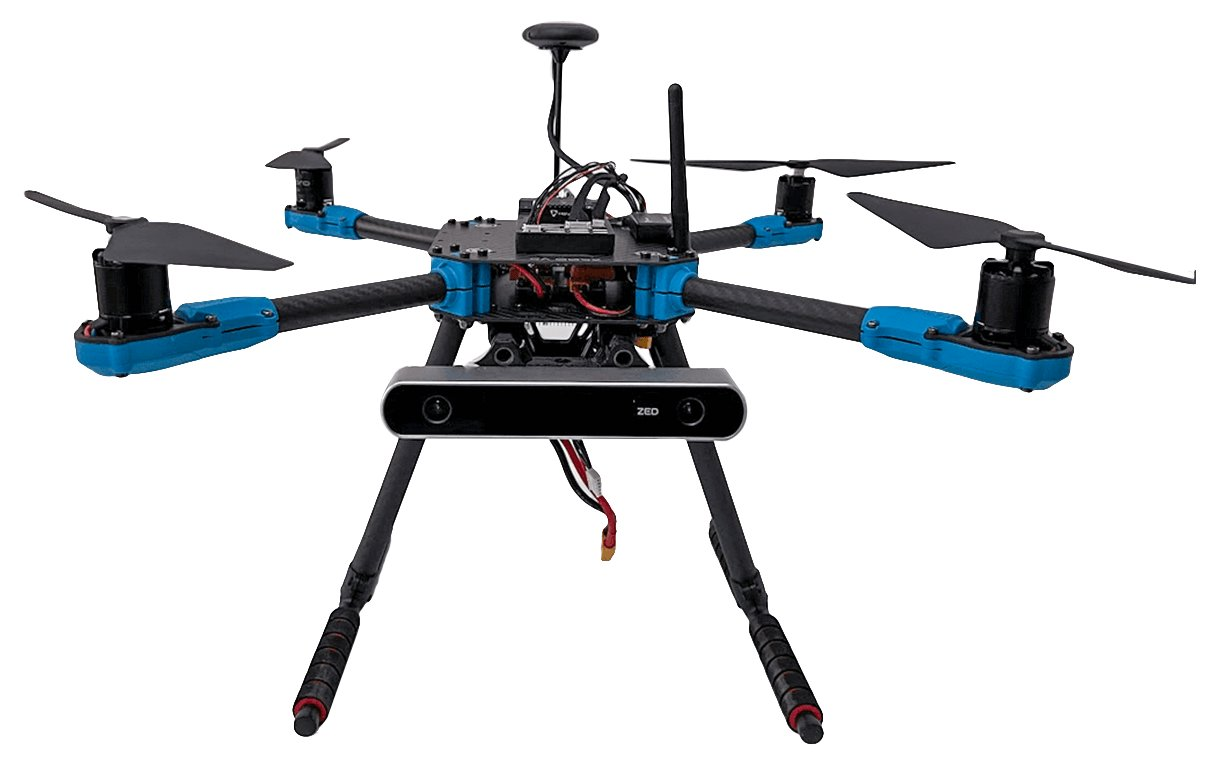
\includegraphics[width=\linewidth]{x500v2_armado}\\
    \credito{Holybro X500 V2. Documentación de PX4 (CC BY 4.0)}
  \end{columns}
\end{frame}

\begin{frame}{Los motores: número, posición y giro}
  \begin{columns}[c]
    \column{0.47\textwidth}\centering
    \begin{tikzpicture}[scale=1.25]
      \draw[line width=3pt,gray!60] (-1.1,1.1) -- (1.1,-1.1);
      \draw[line width=3pt,gray!60] (-1.1,-1.1) -- (1.1,1.1);
      \fill[gray!40] (-0.35,-0.35) rectangle (0.35,0.35);
      % motor 1: adelante derecha, CCW
      \draw[fill=azulclaro] (1.1,1.1) circle (0.42); \node[font=\small\bfseries] at (1.1,1.1) {1};
      \draw[-{Stealth},azul,thick] (1.1+0.55,1.1) arc (0:300:0.55);
      % motor 2: atrás izquierda, CCW
      \draw[fill=azulclaro] (-1.1,-1.1) circle (0.42); \node[font=\small\bfseries] at (-1.1,-1.1) {2};
      \draw[-{Stealth},azul,thick] (-1.1+0.55,-1.1) arc (0:300:0.55);
      % motor 3: adelante izquierda, CW
      \draw[fill=red!10] (-1.1,1.1) circle (0.42); \node[font=\small\bfseries] at (-1.1,1.1) {3};
      \draw[-{Stealth},rojo,thick] (-1.1+0.55,1.1) arc (0:-300:0.55);
      % motor 4: atrás derecha, CW
      \draw[fill=red!10] (1.1,-1.1) circle (0.42); \node[font=\small\bfseries] at (1.1,-1.1) {4};
      \draw[-{Stealth},rojo,thick] (1.1+0.55,-1.1) arc (0:-300:0.55);
      \draw[-{Stealth},thick,verde] (0,0) -- (0,0.9) node[above,font=\tiny] {x (frente)};
      \draw[-{Stealth},thick,rojo] (0,0) -- (0.9,0) node[right,font=\tiny,yshift=-6pt] {y (derecha)};
    \end{tikzpicture}
    \column{0.5\textwidth}\small
    Del airframe \cmd{4001\_gz\_x500} (en metros, marco FRD):
    \begin{center}\scriptsize
      \begin{tabular}{cccc}
        \toprule
        Motor & x & y & Giro \\
        \midrule
        1 & $+0.13$ & $+0.22$ & {\color{azul}antihorario} \\
        2 & $-0.13$ & $-0.20$ & {\color{azul}antihorario} \\
        3 & $+0.13$ & $-0.22$ & {\color{rojo}horario} \\
        4 & $-0.13$ & $+0.20$ & {\color{rojo}horario} \\
        \bottomrule
      \end{tabular}
    \end{center}
    \footnotesize Si en el dron real dos motores están cruzados, \textbf{se voltea al despegar}: para eso es
    \cmd{motor\_test}.
  \end{columns}
\end{frame}

\begin{frame}{Los motores en el x500 de la simulación}
  \begin{columns}[c]
    \column{0.5\textwidth}\centering
    \begin{tikzpicture}
      \node[anchor=south west,inner sep=0] (img) at (0,0) {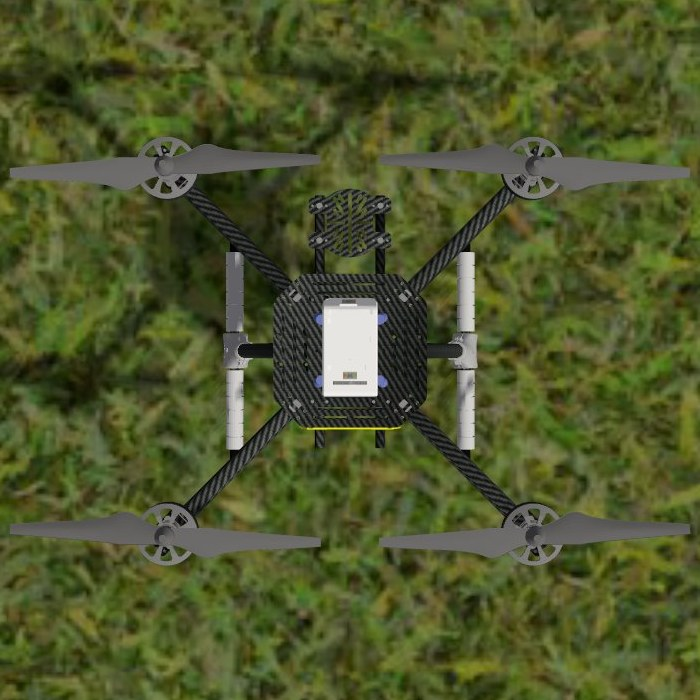
\includegraphics[height=0.72\textheight]{x500_arriba_recorte}};
      \begin{scope}[x={(img.south east)},y={(img.north west)}]
        \node[circle,fill=azul,text=white,font=\bfseries,inner sep=2.5pt] at (0.757,0.771) {1};
        \node[circle,fill=azul,text=white,font=\bfseries,inner sep=2.5pt] at (0.236,0.25) {2};
        \node[circle,fill=rojo,text=white,font=\bfseries,inner sep=2.5pt] at (0.236,0.771) {3};
        \node[circle,fill=rojo,text=white,font=\bfseries,inner sep=2.5pt] at (0.757,0.25) {4};
        \draw[-{Stealth},line width=2pt,verde] (0.5,0.62) -- (0.5,0.93);
        \node[font=\scriptsize\bfseries,verde,fill=white,inner sep=1pt] at (0.5,0.965) {FRENTE};
      \end{scope}
    \end{tikzpicture}\\
    \credito{Render propio de Gazebo, vista desde arriba}
    \column{0.47\textwidth}\centering
    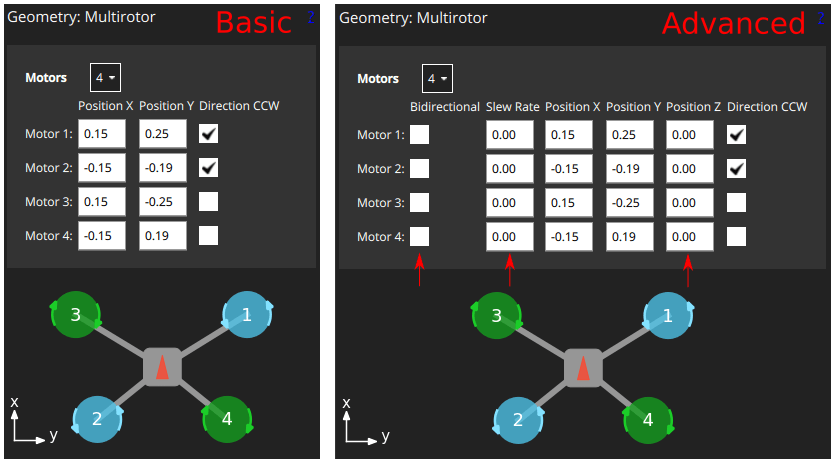
\includegraphics[width=\linewidth]{qgc_motores}\\
    \credito{QGroundControl. Docs de PX4 (CC BY 4.0)}\\[0.4em]
    \raggedright\small Mismo orden en el modelo de Gazebo, en el airframe y en QGC: {\color{azul}azul}
    antihorario, {\color{rojo}rojo} horario.
  \end{columns}
\end{frame}

\begin{frame}{¿Por qué la mitad gira al revés?}
  \begin{columns}[c]
    \column{0.55\textwidth}\small
    Cada hélice que gira empuja hacia arriba \textbf{y} tuerce el cuerpo en sentido contrario (par de
    reacción).
    \begin{itemize}
      \item Dos giran a un lado y dos al otro: los pares se \textbf{cancelan} y el dron no gira solo.
      \item Para \textbf{girar} (yaw), PX4 acelera un par y frena el otro: el empuje total es el mismo,
        pero los pares ya no se cancelan. Acelerar los antihorarios (1, 2) tuerce el cuerpo en sentido
        horario: yaw a la derecha.
    \end{itemize}
    \column{0.42\textwidth}
    \begin{idea}
      \small En el airframe esto es \cmd{CA\_ROTORn\_KM}: $+0.05$ gira antihorario, $-0.05$ horario. El
      \emph{control allocation} lo usa para repartir el giro.
    \end{idea}
  \end{columns}
\end{frame}

\begin{frame}{Cómo se mueve un cuadricóptero}
  \centering
  \begin{tikzpicture}[scale=0.55]
    \begin{scope}[shift={(0,0)}]
      \draw[line width=1.5pt,gray!60] (-1,1) -- (1,-1); \draw[line width=1.5pt,gray!60] (-1,-1) -- (1,1);
      \foreach \p in {(1,1),(-1,-1),(-1,1),(1,-1)} \fill[naranja] \p circle (0.38);
      \node[font=\tiny,align=center] at (0,-1.9) {\textbf{Subir}\\los 4 más rápido};
    \end{scope}
    \begin{scope}[shift={(4.5,0)}]
      \draw[line width=1.5pt,gray!60] (-1,1) -- (1,-1); \draw[line width=1.5pt,gray!60] (-1,-1) -- (1,1);
      \fill[naranja] (-1,1) circle (0.38); \fill[naranja] (-1,-1) circle (0.38);
      \fill[gray!40] (1,1) circle (0.38); \fill[gray!40] (1,-1) circle (0.38);
      \node[font=\tiny,align=center] at (0,-1.9) {\textbf{Roll} a la derecha\\izquierdos más rápido};
    \end{scope}
    \begin{scope}[shift={(9,0)}]
      \draw[line width=1.5pt,gray!60] (-1,1) -- (1,-1); \draw[line width=1.5pt,gray!60] (-1,-1) -- (1,1);
      \fill[naranja] (-1,-1) circle (0.38); \fill[naranja] (1,-1) circle (0.38);
      \fill[gray!40] (1,1) circle (0.38); \fill[gray!40] (-1,1) circle (0.38);
      \node[font=\tiny,align=center] at (0,-1.9) {\textbf{Pitch} adelante\\traseros más rápido};
    \end{scope}
    \begin{scope}[shift={(13.5,0)}]
      \draw[line width=1.5pt,gray!60] (-1,1) -- (1,-1); \draw[line width=1.5pt,gray!60] (-1,-1) -- (1,1);
      \fill[naranja] (1,1) circle (0.38); \fill[naranja] (-1,-1) circle (0.38);
      \fill[gray!40] (-1,1) circle (0.38); \fill[gray!40] (1,-1) circle (0.38);
      \node[font=\tiny,align=center] at (0,-1.9) {\textbf{Yaw} a la derecha\\los antihorarios (1, 2) más rápido};
    \end{scope}
  \end{tikzpicture}
  \vspace{0.4em}

  \raggedright\small Un multicóptero solo puede \textbf{inclinarse} y \textbf{empujar hacia ``arriba''} (de su cuerpo).
  Para avanzar se inclina: parte del empuje apunta hacia adelante.
\end{frame}

\begin{frame}{Los sensores}
  \centering\small
  \begin{tabular}{llll}
    \toprule
    Sensor & Mide & Frecuencia típica & Topic de ROS 2 \\
    \midrule
    Giroscopio & velocidad de giro (rad/s) & cientos de Hz & \cmd{/fmu/out/sensor\_combined} \\
    Acelerómetro & aceleración (m/s$^2$) & cientos de Hz & \cmd{/fmu/out/sensor\_combined} \\
    Barómetro & presión $\rightarrow$ altura & \textasciitilde50 Hz & (no expuesto) \\
    Magnetómetro & campo magnético $\rightarrow$ norte & \textasciitilde50 Hz & (no expuesto) \\
    GPS & latitud, longitud, altitud & 5--10 Hz & \cmd{/fmu/out/vehicle\_gps\_position} \\
    \bottomrule
  \end{tabular}
  \vspace{0.5em}
  \begin{idea}
    \small En SITL los \textbf{simula Gazebo} con ruido; PX4 los recibe por \cmd{gz\_bridge} como si fueran
    reales. Por eso el GPS de la simulación ``se mueve'' unos centímetros aunque el dron esté quieto.
  \end{idea}
\end{frame}

\begin{frame}{EKF2: de sensores a ``dónde estoy''}
  \begin{columns}[c]
    \column{0.5\textwidth}\centering
    \begin{tikzpicture}[node distance=0.25cm,every node/.style={font=\tiny},
        sn/.style={draw=gray,fill=gray!10,rounded corners,minimum width=1.6cm}]
      \node[sn] (i) {IMU};
      \node[sn,below=of i] (b) {barómetro};
      \node[sn,below=of b] (m) {magnetómetro};
      \node[sn,below=of m] (g) {GPS};
      \node[draw=azul,fill=azulclaro,rounded corners,minimum height=2.3cm,minimum width=1.4cm,right=1cm of b,yshift=-0.4cm] (e) {EKF2};
      \foreach \n in {i,b,m,g} \draw[-{Stealth}] (\n.east) -- (e.west);
      \node[draw=azul,rounded corners,right=0.7cm of e,align=left,font=\tiny] (o) {vehicle\_attitude\\vehicle\_local\_position\\vehicle\_global\_position};
      \draw[-{Stealth}] (e) -- (o);
    \end{tikzpicture}
    \column{0.47\textwidth}\small
    \begin{itemize}
      \item Un \textbf{filtro de Kalman extendido}: combina sensores que se equivocan de formas distintas.
      \item La IMU es rápida pero se desvía; el GPS es lento pero no se desvía: juntos dan una
        posición buena y rápida.
      \item Lo que leemos en ROS 2 (\cmd{vehicle\_local\_position}\ldots) es la \textbf{estimación}, no
        el sensor crudo.
    \end{itemize}
  \end{columns}
\end{frame}

\begin{frame}{La cadena de control (en cascada)}
  \centering
  \begin{tikzpicture}[node distance=0.3cm,every node/.style={font=\tiny},
      ct/.style={draw=azul,fill=azulclaro,rounded corners,minimum height=0.8cm,minimum width=1.55cm,align=center}]
    \node[ct] (p) {posición\\(P)};
    \node[ct,right=of p] (v) {velocidad\\(PID)};
    \node[ct,right=of v] (a) {aceleración\\$\rightarrow$ inclinación};
    \node[ct,right=of a] (at) {actitud\\(P)};
    \node[ct,right=of at] (r) {rate\\(PID)};
    \node[ct,right=of r] (c) {allocation\\$\rightarrow$ motores};
    \foreach \x/\y in {p/v,v/a,a/at,at/r,r/c} \draw[-{Stealth}] (\x) -- (\y);
    \node[below=0.15cm of p] {\textasciitilde50 Hz};
    \node[below=0.15cm of r] {\textasciitilde400+ Hz};
    \draw[decorate,decoration={brace,mirror,amplitude=4pt}] ([yshift=-0.7cm]p.south west) -- ([yshift=-0.7cm]a.south east) node[midway,below=4pt] {lo que mandamos en offboard};
  \end{tikzpicture}
  \vspace{0.6em}
  \begin{itemize}\small
    \item Cada lazo le da su \emph{setpoint} al siguiente: el de posición dice ``ve a 2 m/s'', el de velocidad
      dice ``inclínate 10°'', el de actitud dice ``gira a 1 rad/s''\ldots
    \item Los lazos de adentro son \textbf{más rápidos} que los de afuera.
    \item En offboard nosotros entramos \textbf{arriba}: posición, velocidad o aceleración.
  \end{itemize}
\end{frame}

\begin{frame}{Modos de vuelo (\texttt{nav\_state})}
  \centering\scriptsize
  \begin{tabular}{rll@{\hspace{1.2cm}}rll}
    \toprule
    \# & Modo & Quién manda & \# & Modo & Quién manda \\
    \midrule
    0 & Manual & piloto & 4 & Hold (Loiter) & PX4: quieto en un punto \\
    15 & Stabilized & piloto (nivela solo) & 17 & Takeoff & PX4: despega \\
    1 & Altitude & piloto, PX4 sostiene altura & 18 & Land & PX4: aterriza \\
    2 & Position & piloto, PX4 sostiene posición & 5 & Return (RTL) & PX4: a casa \\
    3 & Mission & PX4: plan de QGC & 21 & Orbit & PX4: círculo \\
    14 & \textbf{Offboard} & \textbf{tu nodo} & 12 & Descend & PX4: baja sin GPS \\
    \bottomrule
  \end{tabular}
  \vspace{0.6em}
  \raggedright\small
  \begin{itemize}
    \item En los ejemplos se compara con las constantes: \cmd{VehicleStatus::NAVIGATION\_STATE\_OFFBOARD}.
    \item \cmd{flight\_mode\_monitor} los imprime cada vez que cambian.
  \end{itemize}
\end{frame}

\begin{frame}{Dos maneras de mandar}
  \begin{columns}[t]
    \column{0.48\textwidth}
    \begin{idea}[title={\small\bfseries Offboard},coltitle=black,colbacktitle=azulclaro]
      \small Tu nodo calcula un \textbf{setpoint} 10--20 veces por segundo (posición, velocidad\ldots).
      \begin{itemize}
        \item Control fino: trayectorias, seguir algo.
        \item Si el nodo se cae, PX4 entra en \textbf{failsafe}.
        \item \cmd{takeoff\_mission}, \cmd{square\_mission}, \cmd{orbit\_mission}, \cmd{figure\_eight},
          \cmd{velocity\_control}.
      \end{itemize}
    \end{idea}
    \column{0.48\textwidth}
    \begin{idea}[title={\small\bfseries Comandos},coltitle=black,colbacktitle=azulclaro]
      \small Tu nodo manda \textbf{órdenes}: despega, ve a, orbita, regresa. PX4 vuela con sus modos.
      \begin{itemize}
        \item Menos código, más seguro: si el nodo se cae, PX4 sigue.
        \item Menos control fino.
        \item \cmd{orbit\_command}, \cmd{goto\_mission}, \cmd{return\_home}, \cmd{change\_speed},
          \cmd{set\_home}.
      \end{itemize}
    \end{idea}
  \end{columns}
\end{frame}

\begin{frame}{Armar}
  \begin{columns}[c]
    \column{0.55\textwidth}\small
    \textbf{Armar} = darle permiso a los motores de girar. Antes, PX4 corre los \textbf{preflight checks}:
    \begin{itemize}
      \item sensores calibrados y coherentes, EKF2 convergido,
      \item GPS con fix (si el modo lo necesita), batería suficiente,
      \item enlace con la estación de tierra (\cmd{NAV\_DLL\_ACT}),
      \item el modo pedido se puede usar ahora.
    \end{itemize}
    Si algo falla, rechaza el armado y lo dice en la consola y en QGC.
    \column{0.42\textwidth}
    \begin{terminal}{consola de PX4}
WARN Preflight Fail:\\
\ \ ekf2 missing data\\
WARN Preflight Fail:\\
\ \ No connection to the GCS\\
WARN Arming denied: Resolve\\
\ \ system health failures first
    \end{terminal}
    \small Al tocar tierra, PX4 \textbf{desarma solo} (unos segundos después).
  \end{columns}
\end{frame}

\begin{frame}{Failsafes}
  \small Cuando algo sale mal, PX4 toma el control y hace una acción configurada:
  \vspace{0.3em}
  \centering\scriptsize
  \begin{tabular}{lll}
    \toprule
    Situación & Parámetro & Acción típica \\
    \midrule
    Se dejan de recibir setpoints de offboard & \cmd{COM\_OF\_LOSS\_T}, \cmd{COM\_OBL\_RC\_ACT} & Hold / Return / Land \\
    Se pierde la estación de tierra & \cmd{NAV\_DLL\_ACT} & Return \\
    Batería baja / crítica & \cmd{BAT\_LOW\_THR}, \cmd{COM\_LOW\_BAT\_ACT} & aviso / Return / Land \\
    Se sale de la geocerca & \cmd{GF\_ACTION} & aviso / Hold / Return \\
    Se pierde el control remoto & \cmd{NAV\_RCL\_ACT} & Return \\
    \bottomrule
  \end{tabular}
  \vspace{0.4em}
  \raggedright
  \begin{idea}
    \small \cmd{/fmu/out/failsafe\_flags} trae una bandera por cada cosa que PX4 vigila; \cmd{flight\_mode\_monitor}
    las muestra.
  \end{idea}
\end{frame}

\begin{frame}[fragile]{Parámetros de PX4 (no son los de ROS)}
  \small PX4 tiene \textasciitilde1000 parámetros propios: ganancias, límites, alturas. Se ven y cambian en
  QGroundControl (Vehicle Setup $\rightarrow$ Parameters) o en la consola \cmd{pxh>}:
  \begin{lstlisting}[style=bash,caption={En la terminal donde corre PX4 SITL}]
pxh> param show MIS_TAKEOFF_ALT        # altura del modo Takeoff
pxh> param show MPC_XY_VEL_MAX         # velocidad horizontal máxima
pxh> param set RTL_RETURN_ALT 15       # altura a la que regresa Return
pxh> commander status                  # estado general
pxh> listener vehicle_local_position   # leer un topic uORB
  \end{lstlisting}
  \begin{ojo}
    \small No confundir con los parámetros de ROS 2 de nuestros nodos (\cmd{--ros-args -p radius:=8.0}):
    esos son de tu programa, no de PX4.
  \end{ojo}
\end{frame}

\begin{frame}{La simulación completa}
  \centering
  \begin{tikzpicture}[node distance=0.45cm,every node/.style={font=\tiny},
      bx/.style={draw=azul,fill=azulclaro,rounded corners,minimum height=0.8cm,minimum width=2cm,align=center}]
    \node[bx,fill=gray!15,draw=gray] (gz) {Gazebo Harmonic\\física, sensores};
    \node[bx,right=0.9cm of gz] (px) {PX4 SITL};
    \node[bx,right=0.9cm of px] (ag) {Agente\\Micro XRCE-DDS};
    \node[bx,right=0.9cm of ag,fill=yellow!20] (ros) {Tus nodos\\de ROS 2};
    \node[bx,below=0.8cm of px,fill=gray!15,draw=gray] (qgc) {QGroundControl};
    \draw[{Stealth}-{Stealth}] (gz) -- node[above]{gz\_bridge} (px);
    \draw[{Stealth}-{Stealth}] (px) -- node[above]{UDP 8888} (ag);
    \draw[{Stealth}-{Stealth}] (ag) -- node[above]{DDS} (ros);
    \draw[{Stealth}-{Stealth}] (px) -- node[right]{MAVLink (UDP 14550)} (qgc);
  \end{tikzpicture}
  \vspace{0.6em}
  \begin{itemize}\small
    \item \cmd{vespo up --sim} levanta todo esto: el agente, PX4 + Gazebo y QGroundControl.
    \item \textbf{Lockstep}: PX4 avanza al paso de Gazebo. Si la simulación va lenta, PX4 también; tu
      nodo (con el reloj de la pared) no.
  \end{itemize}
\end{frame}
